\section{Overview of available Direct Sparse Solver (DSS) libraries}


%%%%%%%%%%%%%%%%%%%%%%%%%%%%%%%%%%%%%%%%%%%%%%%%%%%%%%%%%%
\begin{frame}[t]{List of parallel DSSs}
    \small
    
    \begin{table}[!ht]
    	\footnotesize
    	\centering
    	\begin{tabular}{|c|c|c|c|c|}
    		\hline
    		Package & Method             & Matrix Types                 & \multicolumn{1}{c|}{\begin{tabular}[c]{@{}c@{}}PETSc\\ Interface\end{tabular}} & License      \\ \hline
    		Clique       & Multifrontal       & Symmetric      & \multicolumn{1}{c|}{\begin{tabular}[c]{@{}c@{}}Not \\ Officially\end{tabular}} & Open  \\ \hline
    		MF2          & Multifrontal       & \begin{tabular}[c]{@{}c@{}}Symmetric\\ pattern\end{tabular} & No              & -            \\ \hline
    		DSCPACK      & Multifrontal       & SPD                          & No              & Open \\ \hline
    		MUMPS        & Multifrontal       & General                      & Yes             & Open  \\ \hline
    		PaStiX       & Left looking & General                      & Yes             & Open  \\ \hline
    		PSPASES      & Multifrontal       & SPD                          & No              & Open \\ \hline
    		SPOOLES      & Left-looking       & \begin{tabular}[c]{@{}c@{}}Symmetric\\ pattern\end{tabular} & No              & Open \\ \hline
    		SuperLU\_DIST & Right-looking      & General                      & Yes             & Open  \\ \hline
    		symPACK      & Left-Right looking & SPD                          & No              & Open  \\ \hline
    		S+           & Right-lookin       & General                      & No              & -            \\ \hline
    		
    		PARDISO         & Multifrontal       & General                      & No              & Commercial   \\ \hline
    		
    		WSMP         & Multifrontal       & General                      & No              & Commercial   \\ \hline
    	\end{tabular}
    	\caption{A list of direct sparse linear solvers adapted for \\distributed-memory computations, \cite{list-of-sparse-direct-solvers}, \cite{petsc-web-page}}
    	
    	\label{table:mm-library-spec}
    \end{table}
\end{frame}


\begin{frame}[t]{Comparisons of DSSs}
	\begin{figure}[!h]
		\centering
		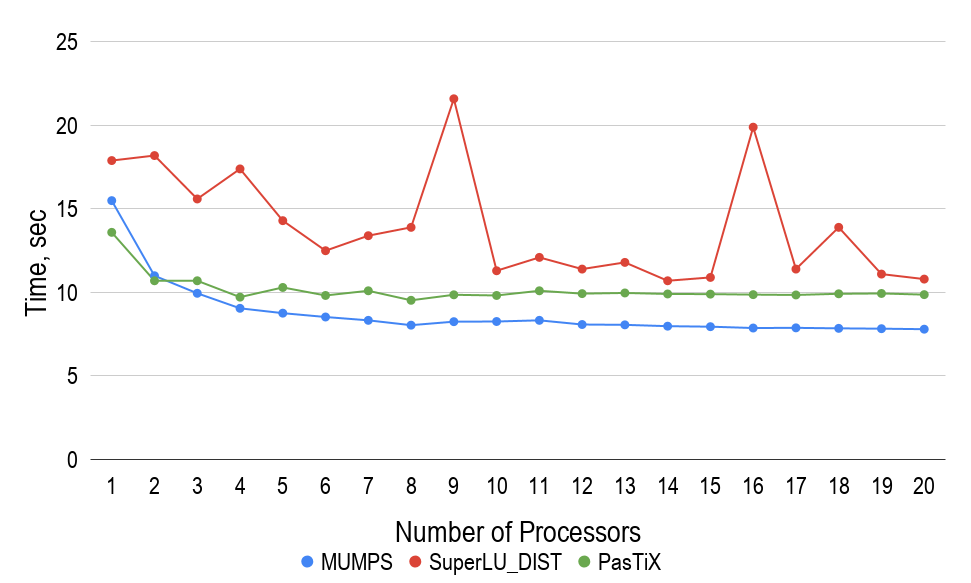
\includegraphics[width=0.875\textwidth]{figures/chapter-2/solvers-comparison-5-point-stencil.png}
		\caption{Comparisons of MUMPS, PasTiX and SuperLU\_DIST libraries during 5 point-stencil Poisson matrix (1000000  equations) factorizations
		}
		\label{fig:5-point-stencil-solvers-comparison}
	\end{figure}
\end{frame}